
\documentclass[11pt,a4paper]{report}
\usepackage{amsmath}
\usepackage{amsfonts}
\usepackage{amssymb}
\usepackage{graphicx}
\usepackage[left=2cm,right=2cm,top=2cm,bottom=2cm]{geometry}
\author{Fermin A. Ahumada Garcia}
\title{Reporte Tarea 2}
\begin{document}
\maketitle
\section*{Problema 5 }
\textbf{La llamada (bundle ’(”a” ”b” ”c”) 0) es un buen uso de bundle? ¿qué produce? ¿por qué?}\\
Este ejemplo en particular iba generar un bucle infinito, por que al llamar a \textit{drop} y \textit{take}, al ser  $n = 0$,hace que no recorra los elementos de esta,y nunca se vaciará.
\section*{Problema 9}
\textbf{Dibuja un diagrama como el de la figura anterior pero para la lista ’(11 9 2 18 12
14 4 1).}\\
\begin{figure}[ht]
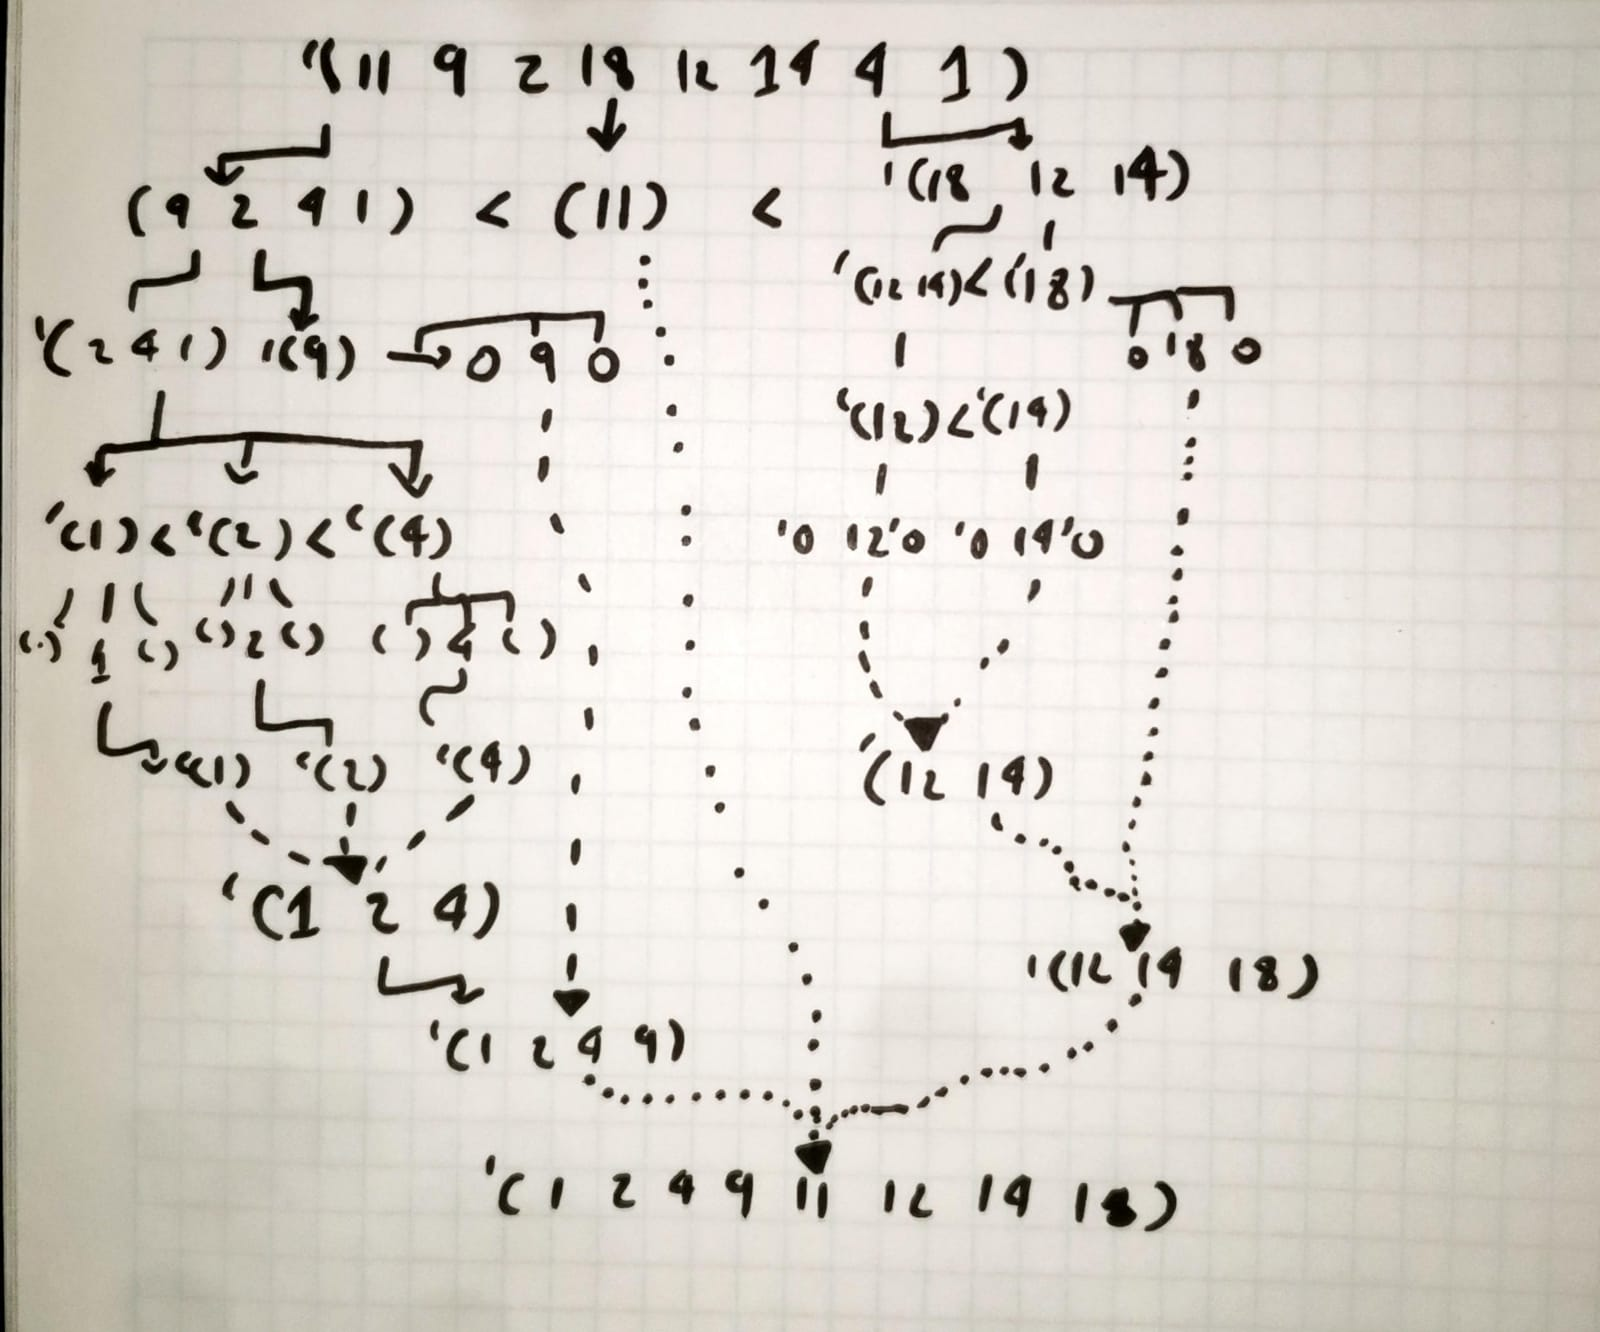
\includegraphics[width=15cm]{image}
\centering
\end{figure}
\section*{Problema 11}
\textbf{Si la entrada a quicksort contiene varias repeticiones de un número, va a regresar una lista estrictamente más corta que la entrada. Responde el por qué y arregla el problema.}

\end{document}